\appendix
\section{Tables}
\subsubsection{Gregor -- Keyboard Shorcuts}
{
    \begin{tabular}{|c|l|}
      \hline
      % after \\: \hline or \cline{col1-col2} \cline{col3-col4} ...
      Key & Action \\
      \hline
      \multicolumn{2}{|c|}{The File Menu} \\
      \hline
      Ctrl + O & Open an existing document \\
      Ctrl + S & Save the document to the last selected file or a new file if no previous file is associated. \\
      Ctrl + Shift + S & Save the data in a new file \\
      Ctrl + I & Import spline data from file \\
      Ctrl + E & Open up the export menu \\
      Shift + Del  & Clear the workspace \\
      Alt + F4 & Close the application \\
      \hline
      \multicolumn{2}{|c|}{The View Menu} \\
      \hline
      Ctrl + 4 & Combined Mode; Shows both ink and curves \\
      Ctrl + 5 & Ink Only Mode; Shows Only the ink marks and hides the curve alogwith the handles \\
      Ctrl + 6 & Splines Mode. Hides the ink marks \\
      Ctrl + G & Toggle the visibility of the grid \\
      Ctrl + Shift B & Toggle the visibility of the background images \\
      \hline
      \multicolumn{2}{|c|}{The Edit Menu} \\
      \hline
      Ctrl + 1 & Toggles the splines anchor centers \\
      Ctrl + 2 & Toggles the splines curvature handles \\
      Ctrl + 3 & Toggles the rotation handles \\
      Ctrl + V & Toggles the action of mouse left click between adding the anchor and dragging the workspace. \\
      \hline
      \multicolumn{2}{|c|}{Help}\\
      \hline
      F1 & Shows quick help \\
      F2 & Opens up the project Git.\\
      \hline
    \end{tabular}\label{Table:Keyboardshortcuts}
}
\clearpage
\section{Source Code}\label{Appendix:sourceCode}
{
\clearpage }
\section{Videos}\label{Appendix:sourceCode}
{
\clearpage }
\section{Code Snippetes}
{
\begin{lstlisting}[language=XML]
//Sample code of a rotating Bezier spline that will render the Urdu letter Aa'en in Nastaleeq.
<spline>
    <FlatTipWidth>150</FlatTipWidth>
    <Color>-5658199</Color>
    <anchor>
      <rotationoffset>0</rotationoffset>
      <P>-198.3791, 452.6993</P>
      <C1>-131.6351, 572.4461</C1>
      <C2>-265.1234, 332.9534</C2>
      <R1>-148.3791, 452.6993</R1>
    </anchor>
    <anchor>
      <rotationoffset>0</rotationoffset>
      <P>-296.5323, 156.2775</P>
      <C1>-439.8357, 254.4304</C1>
      <C2>-119.5302, 35.04326</C2>
      <R1>-246.5322, 156.2775</R1>
    </anchor>
    <anchor>
      <rotationoffset>0</rotationoffset>
      <P>25.40986, 374.1774</P>
      <C1>-47.22344, 262.2825</C1>
      <C2>98.04301, 486.0714</C2>
      <R1>75.40986, 374.1774</R1>
    </anchor>
    <anchor>
      <rotationoffset>0</rotationoffset>
      <P>-233.7143, -183.332</P>
      <C1>-208.1945, -28.25013</C1>
      <C2>-274.7982, -432.9961</C2>
      <R1>-183.7143, -183.332</R1>
    </anchor>
    <anchor>
      <rotationoffset>0</rotationoffset>
      <P>315.9428, -517.0526</P>
      <C1>95.77186, -679.5702</C1>
      <C2>435.6645, -428.6809</C2>
      <R1>365.9427, -517.0526</R1>
    </anchor>
    <anchor>
      <rotationoffset>0</rotationoffset>
      <P>441.5787, -144.0708</P>
      <C1>388.576, -277.5591</C1>
      <C2>494.5813, -10.58265</C2>
      <R1>491.5787, -144.0708</R1>
    </anchor>
  </spline>
\end{lstlisting}
}
\section{Images}
{   

\begin{figure}[H]
  \centering
  \includegraphics[width=0.8\textwidth]{Nastaleeq_Ink.pdf}
  \caption
  {
      Nastaleeq sample by Gohar Qalam. (a) Original calligraphy photo. (b) Original photo processed for analysis. (c) Traced rotating bezier spline ink. (d) Difference between (b) and (c). The red pixel indicate the portions that are missing in (c) but are present in (b) and the blue ones show the missing pixels in (b) but are present in (c).
  }
\end{figure}

\begin{figure}[H]
  \centering
  
\includegraphics[width=0.8\textwidth]{Nastaleeq_Machined.pdf}
  \caption
  {
      Machined Nastaleeq sample by Gohar Qalam. (a) Rasterized rotating bezier spline for machining (b) Ink marks machined by a simulated robotic manipulator. (c) and (d) are differences between simulated ink mark and the rasterized photo and the processed original photo respectively. The red pixel indicate the portions that are missing in (c) but are present in the reference image and the blue ones show the missing pixels in reference but are present in the ink mark.
  }
\end{figure}

\begin{figure}[H]
  \centering
  
\includegraphics[width=0.8\textwidth]{Thuluth_Ink.pdf}
  \caption
  {
      Thuluth sample by Gohar Qalam. (a) Original calligraphy photo. (b) Original photo processed for analysis. (c) Traced rotating bezier spline ink. (d) Difference between (b) and (c). The red pixel indicate the portions that are missing in (c) but are present in (b) and the blue ones show the missing pixels in (b) but are present in (c).
  }
\end{figure}

\begin{figure}[H]
  \centering
  
\includegraphics[width=0.8\textwidth]{Thuluth_Machined.pdf}
  \caption
  {
      Machined Thuluth sample by Gohar Qalam. (a) Rasterized rotating bezier spline for machining (b) Ink marks machined by a simulated robotic manipulator. (c) and (d) are differences between simulated ink mark and the rasterized photo and the processed original photo respectively. The red pixel indicate the portions that are missing in (c) but are present in the reference image and the blue ones show the missing pixels in reference but are present in the ink mark.
  }
\end{figure}
}
\section{Gregor -- The Twisting Bezier Spline Editor}\label{Chapter:Gregor}
\subsection{Introduction}
{
    The twisting Bezier splines may well mathematically be able to quite accurately contain most of the information required to replicate a calligraphy artwork but will hardly be practically useful without a tool strong enough to enable an artist to effectively trace an existing or create a new calligraphy specimen. Now, making such a tool was in itself an entire software engineering project and could not easily fit in the scope of the on going work. However with this link missing, in would have been impossible to quantitatively test and benchmark the performance of the other tools. So the least that could actually be done would be to layout the bare minimum user requirements and start writing the tool. The coding work was only as linear as any other software project which relies on ambiguous and equivocal requirements. Meaning that once the first version of the software had been built, the software had to be taken back to development many times after tests with real artists. Some features were added later to fulfil the necessity that was felt during the trial while others which were initially considered to be cardinal to working of the application.

    The name ``Gregor'' is taken from a character of George R. R. Martin's legendary novel\cite{bib19} series Game of thrones. He is one of his kind; not the fastest fighter there is but is strong and every blow of his sword is effective.

    Once the application had been developed, came another step which is often forgotten and considered dispensable usually by most developers; documenting the code and the usage. Documentation of the code and a user manual is the only thing that turns an application into a software. As said earlier, keeping in view the scope of the project, the documentation too had to be limited to contain only the most critical parts. This chapter may serve as the user manual of the software. The user guide includes:
    \begin{itemize}
      \item describing how the application should be used normally,
      \item the user interface,
      \item keyboard shortcuts,
      \item saving and loading data, and
      \item introduction to analysis tools.
    \end{itemize}
    While the coding manual includes:
    \begin{itemize}
      \item general code organization,
      \item architecture and functionality of the most important parts of the code, and
      \item the relationships between most significant entities.
    \end{itemize}
    Additionally, some snippets of the code are also included in the printed appendix and in addition to uploading the whole code as a Github repository \cite{bib20}, it can be found in appendix B which is a memory card that can be access by most computers and smart-phones.
}
\subsection{Requirements and Features}
{
    The most fundamental user requirements are very simple.
    \begin{itemize}
      \item
      {
        The most fundamental requirement was that the tool be able to let the user graphically draw a rotating bezier spline. It was not only convenient but also logical to make the editing sequence similar to other vector editing software. This will make the transfer easier for people who already have some experience in other applications.
      }
      \item
      {
        The application must be able to save and load the edited work using a data file.
      }
      \item
      {
        The user should be able to drag and zoom the view port using the mouse cursor and keyboard shortcuts.
      }
      \item
      {
        There should be a provision to load images into the workspace so that they can be traced.
      }
    \end{itemize}

    Additionally, from a developer's perspective there are some features that are either implemented inevitably along the way of implemented the essential features or the usability of these features outweighs the additional effort required for the implementation. For example, the developer would have to program at least one color that the view-port will use to visualize the splines. The effort required to just expose the color option to the user is negligible as compared to writing the rendering engine. Many such features were also made a part of Gregor.

    \begin{itemize}
    \item Toggling the visibility of curvature and rotation handles.
    \item Toggling the visibility of ink-marks.
    \item Changing the opacity and color ink-marks.
    \item Changing the viewing mode between editing and viewing.
    \item Grid snapping with an option to be toggled on or off.
    \item Changing the rendering mode of rotating bezier splines.
    \item Selecting, moving, deleting, hiding and enabling individual splines.
    \item Document explorer with thumbnails of every spline in the document.
    \item Importing splines into existing workspace
    \item Selecting, moving, deleting, hiding and enabling individual splines.
    \item Application menu to change options with keyboard shortcuts to most used menu items
    \end{itemize}
}
\subsection{Usage}
{
    The software can be used to create/trace new splines and also open up existing ones. The software uses Microsoft XML format to store data. While creating or editing a spline, the user adds more anchors by clicking on the desired position on the document. Anchors can be added to previous splines as well as the one under focus. Once a spline has been created, the user can change the thickness and color of the ink-mark and then fine tune the position of each anchor point to match the desired stroke. To trace the strokes of an existing document, the user can also load images on to the background of the document and resized and positioned at the desired position.

    Once some splines have been created, the user can choose to save the work as XML documents or be exported as images. The user can also compare the newly created artwork with the background images to analyze the false positive and false negative areas. The analysis tools can preview the difference and compute the number of pixels in each difference image.
}
\subsection{Interface}
{
    The view of the software is the spline editor with a detailed main menu as shown in Fig. \ref{Fig:GregorInterface}, document summary and a list of most commonly used toggle buttons. The application also provides some keyboard shortcuts for the most frequently used toggle options like changing the visibility of different elements and toggling the editing modes.

    The information a rotating spline contains is too much to be viewed simultaneously. The center point of the anchors, the curvature handles, twist handles, the curve, the inkmark and the background image, when displayed simultaneously is just chaotic. On top of that, when all of these elements are interactive, using a single mouse cursor to interface becomes a headache. This is why the application presents viewing and editing modes.
    \subsubsection{The Viewing Modes}
    {
        The viewing modes can be controlled using options (g1) through (g3) as shown in Fig.  \ref{Fig:GregorInterface}, the ``View'' menu (a2), or the keyboard shortcuts. There are essentially three modes of view.
        \begin{itemize}
          \item (g1) is ink and curve mode. In this mode, the splines curves and the selected handles will be shown alongwith the ink marks.
          \item (g2) is ink-only mode. In this mode, the curvature handle of the splines alongwith the anchors and the handles are hidden.
          \item (g3) is curve-only mode. The inkmark will be hidden in this mode and only the curve alongwith the selected handles will be visible.
        \end{itemize}
        it is obvious that only one mode can be activated at a moment and it can be selected either from the options (g1) through (g3) in Fig.  \ref{Fig:GregorInterface} or through the View menu. Instead of clicking on the toggle buttons, using the keyboard shortcuts can sometimes be even more convenient.
    }
    \subsubsection{The Editing Modes}
    {
        The editing models enable or disable the anchors, curvature handles and the twist handles. As shown in Fig. \ref{Fig:GregorInterface} (h1) through (h3), the editing mode toggle buttons can be used to enable or disable any of these handles. Just like the editing modes, these modes can also be controlled using the keyboard shortcuts. Unlike the viewing modes, however, these modes can be enabled all at a time. It must be noted that while in ink-only mode, none of the editing modes will have any effect of the usability of the editing handles.
    }

    \begin{figure}
      \centering
      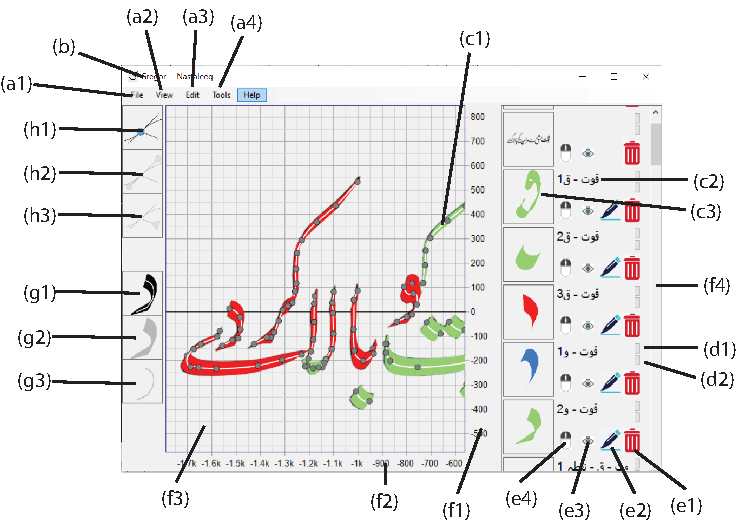
\includegraphics[width=0.9\textwidth]{GregorInterface.pdf}
      \caption{(a1-a4) The main menu options: (a1) Contains the options to open, save, import, export and clear splines and background images, (a2) enlists some viewing options; the ink viewing modes, visibility different elements of the workspace, visibility of background images, opacity of the ink-marks and rendering algorithm (a3) contains options related to editing on the workspace. It has the option to change the spline editing modes, the behaviour of left click on the workspace, and whether the splines can be dragged or not. (a4) has some analysis tools. (b) is the name of the currently open document. (c) is the main view of each spline in the document, (c2) and (c3) are the name of each spline element and its thumbnail respectively. (d1) and (d2) change the vertical order (z order) of the elements. While hovering the cursor over overlapping splines, the spline with higher position in the list will receive mouse event earlier. (e1), (e2), (e3) and (e4) are used to toggle editability, change visibility, modify color and thickness and delete the respective spline curve respectively. (f1) and (f2) are x and y axis of the workspace. (f3) is the main viewport. (f4) is the list of all the splines and images in the document. (g1) switches the view mode to both spline and inkmark, (g2) changes the viewing mode to ink only. (g3) changes the viewing mode to spline only. (h1), (h2) and (h3) toggle the visibility of center of anchor, curvature handle and the twist handle of the splines.
      } \label{Fig:GregorInterface}
    \end{figure}

}
\subsection{Modifying A Spline Curve}
{
    The application opens up an empty document by default. The first path one may choose to follow is to create new splines. This is done by adding new anchors. Anchors are added by simply clicking on an empty area of the screen. It must be noted that by default, the behaviour of the left mouse click must be switched from the Edit menu or using the keyboard shortcut to enable ``Add anchors using left mouse click''. Once an anchor has been added, adding a second anchor automatically creates a spline between the previously added anchor.
    \subsubsection{Starting a New Curve}
    {
        Since each click will append an anchor at the end of to the current spline, to break the curve and start a new one, some other procedure must be adopted. This can either be done by right clicking on an empty part of the document or toggling the ``Add anchors using left mouse click'' option off and quickly using the keyboard shortcut.
    }
    \subsubsection{Appending to a Previously Active Curve}
    {
        To append anchors at the end or the beginning of a previously active spline, simple click the center point of the first or the last center of anchor of the desired curve and it will be selected. Now, every new click will append to the selected curve just like before.
    }
    \subsubsection{Adding Anchors in the Middle}
    {
        Unfortunately adding anchor amid a curve is not a possibility yet. It would require an algorithm that can compute the nearest point on a curve from the mouse position that can show where the new anchor will be added. A work-around for now is to add anchors at the beginning or the end and soft the existing anchors inward until one of them reaches the required position.
    }
    \subsubsection{Simultaneous Curve Editing While Adding New Anchors}
    {
        It is usually very convenient to add an anchor while dragging the mouse cursor at the same time. This way, the software first adds an anchor just like it should on a mouse click but by dragging the cursor, instead of dragging the center of the newly added anchor, it drags the respective curvature handle instead. Creating new long strokes is very convenient this way. Please note that for this trick, the viewing mode must be showing the curve and both the centers and curvatures handles should be enabled.
    }
}
\subsection{Modifying an Ink-mark}
{
    \subsubsection{Adding an Ink-Mark}
    {
        Once a spline has been created with two or more anchors, the viewing mode can be switched to show ink and curve and the twist handle can be enabled while disabling the curvature handle. This will not convert the spline to a rotating curve unless it has been given a thickness. To change the thickness of a spline, simply click on it or the respective appearance in the document explorer as shown in Fig. \ref{Fig:AppearanceEditor} (e3). A curve appearance editor will pop up as shown in Fig. . Allowing to change both the broad edge thickness and the color of the ink-mark.

        \begin{figure}
          \centering
          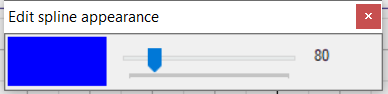
\includegraphics[width=0.3\textwidth]{appearance editor.PNG}
          \caption{The curve appearance editor lets the user modify the color and broad edge thickness of the simulated pen} \label{Fig:AppearanceEditor}
        \end{figure}
    }
    \subsubsection{Modifying the twist/rotation}
    {
        Once the Ink-mark has some thickness, it will start to show up on the viewport as well. If the rotation handles are enabled, one can start dragging each rotation handle to start twisting the curve. The artist usually continuously switches between ink and curvature handles to keep modifying the final spline until they are satisfied with the final ink-marks.
    }
}
\subsection{Using Images}
{
    Images can be imported to an existing workspace by simply selecting the menu option File > Import > Image. One can choose to import an image directly from an image file or the clipboard if the user has already copied an image using a graphics editor like a photoshop or Microsoft Paint. To view it, the background images must also be enabled from the Edit menu. Once the image is visible, the user can select a discrete handle at the middle of the image to change the placement and an anchor at the top right corner to change the size, aspect ratio, mirroring and rotation of the image.
}
\subsection{Using the Document Explorer}
{
    In addition to shoing up in the viewport, all the images and splines also appear in the document explorer as shown in Fig. \ref{Fig:GregorInterface} (f4). Each item is represented by a multi-option control which shows some controls associated with the respective item.
    \begin{itemize}
      \item Fig. \ref{Fig:GregorInterface}(c3) is a normalized thumbnail of the respective item.
      \item One can change the name of each item using Fig. \ref{Fig:GregorInterface}(c2) which can come handy while dealing with multiple items which may look similar.
      \item (e1) will delete the respective item
      \item (e2) pops up the appearance menu of the respective curve
      \item (e3) toggles the visibility of the respective item
      \item (e4) toggles the editability of an item. A Disabled item can be viewed but not interacted with.
      \item (d1) and (d2) change the order of the z-order items in a document. A simple trick while moving an item in a very long list of items is to click once on the required move button and then instead of finding the relocated button again and clicking on it again, one can now choose to press the space bar or the enter button on the keyboard which will press the button again no matter where-ever it is.
    \end{itemize}

}
\subsection{Save, Load, Export}
{
    Once the user is satisfied with the artwork, they can save it using the File menu. Once saved, the user can save any further changes to the same file by simply using the well known save command ``Control + S'' or by using the Save option from the menu again. Once saved, the file can either be opened by using the Open option in the File menu or using the windows explorer. The saved files use an extension ``rbs''. The windows usually does not recognize this extension and will thus present a list of typical applications that can open it. Choose to browse for a custom application and point to the Gregor executable. The windows will not only open the file in Gregor but also remember this choice to open rbs files in the future.

    In addition to opening a file, a user can choose to import the curves contained in a file into an existing workspace, No current items will be cleared while importing a file.

    \subsubsection{Exporting Images}
    {
        Since the curves are vector data, one may still need to export this vector into a rasterized image to be used in various circumstances. A user can export the workspace in a pixel depth of their choice using the export option in the File menu. The export window as shown in Fig. \ref{Fig:ExportMenu} presents several options
        \begin{itemize}
          \item User can control whether to include the anchors and spline curves in the render
          \item The background images can also be exported alongwith the splines.
          \item A uniform color can be selected for the exported splines.
          \item The user can also specify the rendering algorithm for the ink-mark.
          \item Last but not the least, the user can specify a pixel density. By default, each unit on the grid will be considered one pixel. Specifying a pixel density of $100$~DPU specifies to generate one hundred pixels between one unit on the grid. It must be noted that while using too dense or too large images, the application might succumb to the memory load of the procedure. So it is wise to always save the data before attempting to export an image.
        \end{itemize}

        \begin{figure}
          \centering
          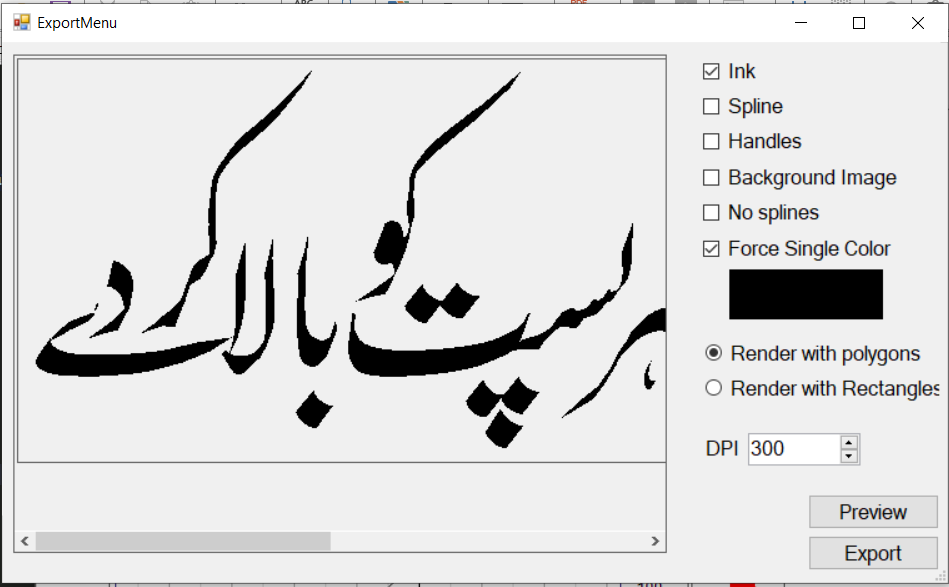
\includegraphics[width=0.9\textwidth]{ExportMenu.PNG}
          \caption{The curve appearance editor lets the user modify the color and broad edge thickness of the simulated pen} \label{Fig:ExportMenu}
        \end{figure}
    }
    \subsubsection{The File Format}
    {
        Gregor uses Microsoft XML format to save data. XML is primarily used to save text data. To pack images in it, the image is first converted into a hexadecimal list of byte data and represented as a very long string. It may inconvenience the user if they try to open it using a simple text editor which will show thousands of lines of gibberish hexadecimal bytes. One way to open the file as text is to open using an advanced raw text editor like Notepad++ or Sublime Text. These editors have the provision to collapse a certain node of an XML document, making the rest of the data more readable.
    }
}
\subsection{Short-keys}
{
    The most common keyboard shortcuts can be viewed in Table \ref{Table:Keyboardshortcuts}.
}
\subsection{Analysis Tools}
{
}
\subsection{Development}
\subsubsection{Code Organization}
\subsubsection{The BezierBoard Class}
\subsubsection{RBSPoint}
\subsubsection{Spline Elements}
\subsubsection{Miscellaneous Helper classes and form}
\subsubsection{Areas needing Improvement}

\clearpage
\section{Drogon -- The Robot Simulator}\label{Chapter:Drogon}
{
    \subsection{Introduction}

    To effectively analyze and verify the proposed solutions, a real robot was needed. Unfortunately with the COVID-19 situation, making a real robot became almost impossible with all the supply shortages and supply chain disturbances. Simulating the manipulator becomes the second option in this case. Although its not a definitive answer but with careful assumptions, a simulator ca very well be used to verify the proposals.

    A lot of effort goes behind only the software design of the simulator but ironically, in the context of the research, it is only supposed to verify whether a robot could use the twisting bezier splines to mimic the hands of an artist. This is why a lot of doors are left open for further development like implementation of other kinds of manipulators and actuators and the usage of the manipulator as a control unit for an actual robot.

    On a lighter note, just like the name Gregor, \textbf{Drogon} was also taken from a fictional character in one of the George R. R. Martin's Game of thrones novels; a mighty dragon.

    \subsubsection{The Requirements}
    Another problem was finding the best simulator to carry out the task. With no earlier training in simulators but a years of experience in programming, I decided to program an in-vitro simulator. The simulator was required to posses some important features and requirements.

    \textbf{The Simulator:}
    \begin{itemize}
      \item Simulate the position and links of the manipulator in discrete time domain.
      \item Simulate the output motors and actuators
      \item PID controllers
      \item Simulate the effect of gravity
      \item Angular and linear momentum
    \end{itemize}

    \textbf{Analysis Tools:}
    \begin{itemize}
      \item $3$~D visualizer
      \item Plotting
      \item Workspace optimizer
      \item Export data for further analysis
      \item Path planner
      \item Manual motor control
      \item Manual end effector control
      \item Machine codes parser
    \end{itemize}

    Out of all these features, there were some that could not be completed or had to be skipped given the scope of the work. Since one may be very tempted to code them or even use them, the doors to implement them are open in the code. The features are as following:
    \begin{itemize}
      \item PID controller (partly implemented)
      \item Linear and angular momentum (partly implemented)
      \item Machine code parser
    \end{itemize}

    Comprehensiveness is the core attribute of Drogon. It provides, under one screen, the flexibility to introduce an elementary change in the design, like, the maximum speed of an actuator and directly observe the consequences on all of the analysis tools. One can choose to programmatically or manually signal an actuator to move in a particular direction and position, and visualize the outcome in a $3$D preview window. It also integrates with Gregor to support the live editing and visualization of rotating bezier spline curves

    Besides comprehensiveness, our design tool offers a set of powerful analysis tools which enabled us to solve complex robot maneuvers and optimize the solution. Performing mechanical simulation with simplified real world constraints, $3$D live preview of the moving robot, work-space optimizer, $2$D art drawing, investigating the actuator velocity in continuous and discrete demain are some of the tools we used for optimization in our design.

    Since the tool is based on in-vitro coding, it can be taught to easily integrate with and inside Microcontrollers to practically , Proteus and SolidEdge to give more design flexibility.

    \subsection{The working principal}
    In this section we discuss the working principals of different aspects of the simulator.

    \subsubsection{Simulation}
    The simulator used in this work is designed from scratch. It is highly customizable in terms of coding and usage. In one configuration it can simulate a manipulator based on steppers motors. This way, the complexity of implementing the effect of gravitational and reactional forces on each actuator. In another configuration, it can simulate actuators with a limited output power, torque/force, response time and even a feedback mechanism making them essentially servo actuators. Not all of the actuators have to this way and the governing limits can also be changed at run-time. Just like the first one, in this configuration too, it first uses forward kinematics of the robot to find out the required position of its actuators to achieve a particular end-effector position and orientation. Unlike stepper motors that can just take a required number of steps in a limited time to achieve a certain position regardless of the load it has to carry, for a servo actuator, the simulator has to calculate the gravitational loads on individual links and propagate the forces and torques to individual actuator. The controller of the actuator is, in parallel, deciding how much output it must produce. Once the simulator has both the forces on each joint, it can calculate the accelerations. And once the accelerations are calculated, it only needs to be integrated with each \emph{tick} of the simulator to yield velocity and position of the actuator. At this point, it may become quite clear that implementing the gyroscopic effects of the links become quite a challenge. Since the robot being analyzed is not supposed to be working at high speeds and loads, the error caused by ignoring this effect in approximation would be negligible.

    \subsubsection{Motor controller}
    One can choose to use either a stepper motor or a DC servo on every joint. In case of stepper motors, one can configure:
    \begin{itemize}
      \item number of steps per revolution, and
      \item minimum step time.
    \end{itemize}
    In this case the simulator assumes:
    \begin{itemize}
      \item the step time remains the same regardless of the motor speed, and
      \item the motor can take a step regardless of the applied load.
    \end{itemize}
    While in case of a servo motor one can configure:
    \begin{itemize}
      \item the maximum input electrical power,
      \item the maximum torque,
      \item maximum idle acceleration,
      \item maximum velocity, and
      \item the \emph{P}, \emph{I} and \emph{D} parameters of the controller.
    \end{itemize}
    In this case, the simulator assumes that:
    \begin{itemize}
      \item the motor are $100$~% energy efficient,
      \item they are weightless, as in they are installed in the base of the robot with mechanical links transferring the power through the arm,
      \item at a constant power, the torque reduces inversely with speed ($Power = torque \times speed$), and
      \item the PID controllers operate independently.
    \end{itemize}

    Moreover, the PID controllers work on a very simple equation
    Later on, it was discovered that implementing simple PID controllers that take the required position as reference were not very effective. So the actuators are kept as stepper motors by default and can be changed to servo motors. Work is still needed to either fine tune the PID controllers or even run them on a more powerful controller.

    More details on the working principles of the simulator will be discussed in later chapters. Also, the installation and usage of the tool is described in detail in Appendix B.

    \subsubsection{Workspace}
    The workspace contains a spherical manipulator as discussed in chapter \ref{chapter2}. The simulator considers the robot fixed on a horizontal surface at the origin $(0, 0, 0)$ with the first link along the vertical axis.

    \subsection{About the Tools}

    An shape independent model of the robot under simulation can be visualized in real time using ``$3D$ Animation'' tool as seen in Fig. \ref{Fig3D}. The ``Robot Feet Position'' tool gives a superior insight on the stability of the robot. It can be seen in Fig. 1A(e) that the center of gravity plot can help optimize the motion where stability is a concern. Using the trajectory of the center of the robot in the global frame of reference can help determine the most efficient actuator movements which can be used to displace the robot from a specific position. Screen shots of the plot produced using the ``Top Trajectory'' tool can be seen in Fig. 1A(d).


        \begin{figure}
          \centering
          \includegraphics[width=0.7\textwidth]{3D.png}
          \caption{A screenshot of the $3$D representation tool. The blue sphere under the end effector shows the target given to the robot.
          } \label{Fig3D}
        \end{figure}

    All of the tools can output in real time. The robot configuration and other parameters change with time, producing animations which make it easier to decipher the underlying information.

    \subsection{Workspace Optimization}
    The workspace optimizer allows to simulate the robot solution recursively through discrete sections of the defined workspace and evaluates the degrees of freedom the robot has  specific parts of the workspace. It then colors the segments to give a more clear idea of the robot workspace. The user can then modify the robot and see, in-result, the change in the workspace. A typical output of the workspace is show in Fig.

        \begin{figure}
          \centering
          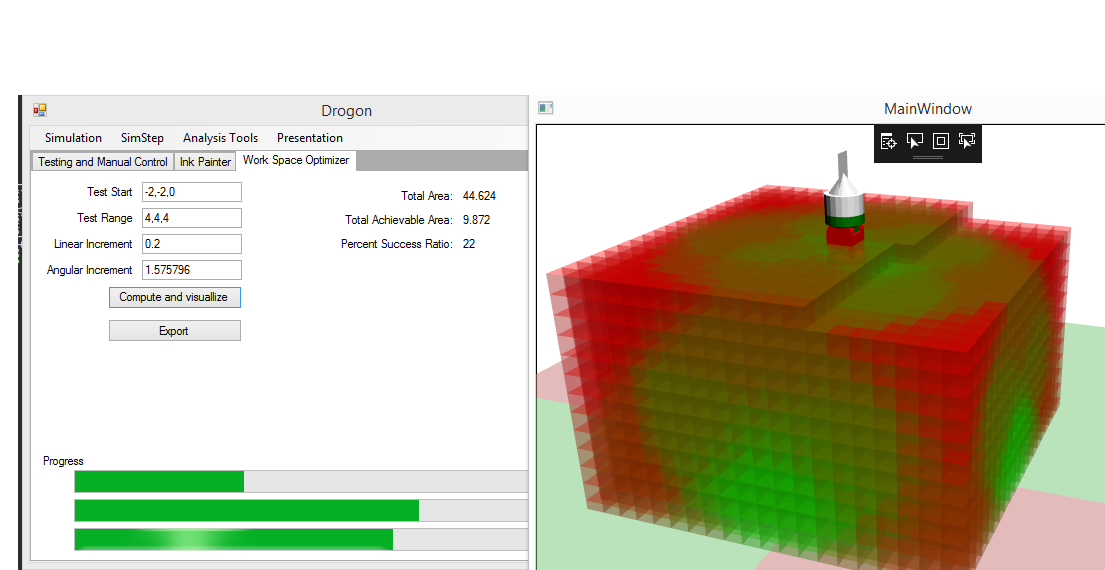
\includegraphics[width=0.9\textwidth]{WorkSpaceOptimer.png}
          \caption{The workspace is coded in colors. Purely green blocks represent a point where the robot has all of the degrees of freedom and the slightly red blocks indicate the parts where robot starts to loose one or more degrees of freedom.
          } \label{FigWorkspace}
        \end{figure}
    \subsection{Script Path Planner}
    As already mentioned, I've included a tool to construct bezier rotation splines in the tool which can serialize the data in computer files and also load from existing files. A screenshot can be seen in Fig.

        \begin{figure}
          \centering
          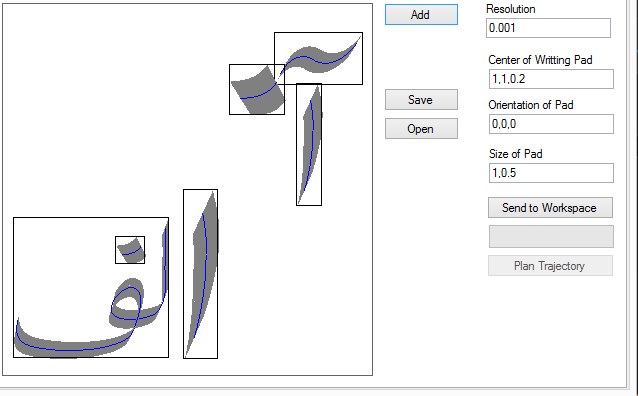
\includegraphics[width=0.9\textwidth]{SctiptEditor.png}
          \caption{The script maker can manage multiple splines and render robot trajectory according to the user resolution requirement.
          } \label{FigWorkspace}
        \end{figure}
    \subsection{Script Motion Simulator}
    Once the script is constructed using the script maker, it can be transported to the workspace in any orientation. The robot then plans how to make the required maneuvers and sibilates the behaviour. A screenshot of a robot writting a script can be seen in figure \ref{FigScriptMotion}
        \begin{figure}
          \centering
          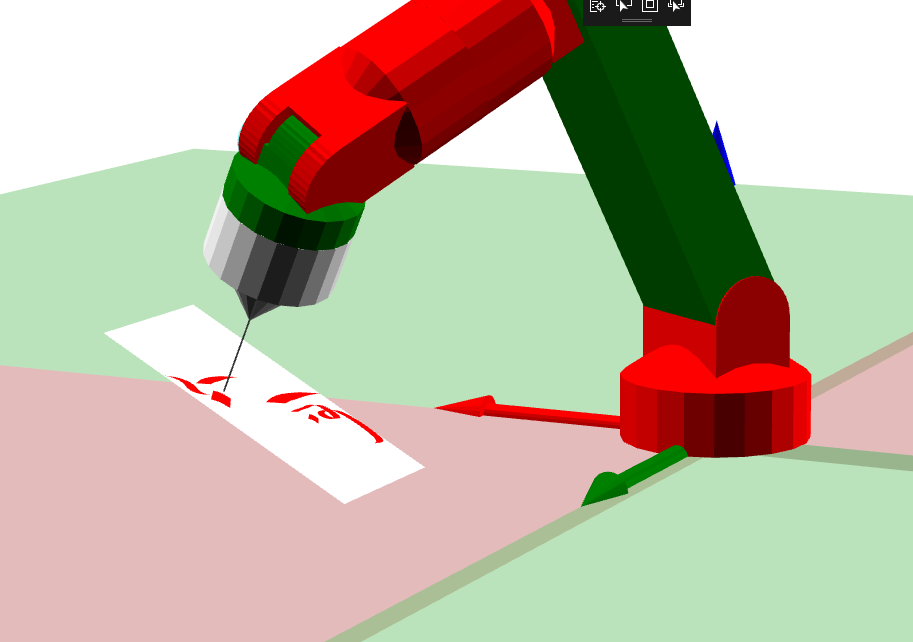
\includegraphics[width=0.9\textwidth]{writting.PNG}
          \caption{Robot writting on a slanted plane.
          } \label{FigScriptMotion}
        \end{figure}
}
\clearpage 